

\subsection{Building Blocks of the Certification Schemes}
\label{bblocks}
Modern certification frameworks rely upon several components defining how the process is executed and how the results should look. Below is a detailed list of the major pillars of certification frameworks with their fundamental functionalities as underlined by Anisetti et al. \cite{anisetti2017semi}\cite{anisetti2022multi}.

\subsubsection{Non-Functional Properties}
For the certification process of a system, it is important to establish some requirements that can be functional or non-functional preemptively, usually this is done during an initial risk assessment process. As stated by Chen et al. \cite{chen2013verification}: ``broadly, functional requirements define what a system is supposed to do, and non-functional requirements define how a system is supposed to be", meaning that non-functional requirements focus on the system itself instead of what the system produces in output; once a requirement is proven to be satisfied by the system, it becomes a non-functional property of the same, and it can be expressed as follows: ⟨name, {(attribute, value), (attribute, value)}⟩. A property is composed of pairs ``attribute-value" where the attributes are essential sub-properties that define the strength of the property. In other words, non-functional properties describe the system's capabilities and are usually grouped under the categories defined by the CIA triad: i) Confidentiality, ii) Integrity and iii) Availability. The CIA triad is an organizational model designed to guide information storing policies; its three parts are cybersecurity's three most crucial components. These properties are considered abstract because they represent generic security requirements and provide no information on how to achieve them. Instead, they are used to define concrete security properties. 

As defined by Anisetti et al. \cite{anisetti2013test}, a concrete security property is formally defined as follows:
A concrete security property, denoted \(p\), is a pair \( ( \hat{p}, A) \), where \(\hat{p}\) is an abstract property and \(A\) is a set of class attributes specifying the threats the service proves to counteract or the specific characteristics of the security function implemented by the service. 

The NIST defined these components as follows \cite{pub2005minimum}:
\begin{description}
    \item[Confidentiality] Preserving authorized restrictions on information access and disclosure, including means for protecting personal privacy and proprietary information. Confidentiality is a set of rules that limits access to information; ensuring confidentiality means the authorized entities can access the protected information and the unauthorized entities cannot. Confidentiality is accomplished through methods like data encryption and authentication procedures.
    \item[Integrity] Guarding against improper information modification or destruction, and includes ensuring information non-repudiation and authenticity. Integrity is the assurance that the information is trustworthy and accurate; it involves maintaining data consistency and accuracy over its entire lifecycle. For example, measures like file permissions and user access control ensure unauthorized entities cannot change data, while checksums and backups safeguard data from non-human threats like electromagnetic pulses or server crashes.
    \item[Availability] Ensuring timely and reliable access to and use of information. Availability guarantees reliable access to the information; it is best ensured by rigorously maintaining all hardware and staying up to date with all system upgrades; providing bandwidth, preventing bottlenecks and fast disaster recovery are also essential.

\end{description}



\subsubsection{Non-Functional Mechanisms}
For a non-functional property to be proven, a non-functional mechanism, in the form of \( ( name, \{ attribute, value \} )\), must be implemented to execute the certification process under specific configurations. Moreover, the property is what the process needs to verify, and the mechanism is the tool the system offers to test such property \cite{anisetti2017semi}; the verification is usually done through tests in the form of \\ \( (mechanism, (codde to execute, expected results))\). Finally, it is important to note that the mechanisms need to be described in the system's documentation; this allows the accredited laboratory to analyze and test them during the manual review phases.


\subsubsection{Target of Certification}
The application context and the system perimeter define the Target of the Certification (ToC); it describes the mechanisms on which the non-functional properties that need to be certified rely. Moreover, the evaluation of the certification scheme must verify the target’s (security) features. For example, in the Common Criteria process, the ToC (actually named Target of Evaluation) is accurately described in the Security Target Document.

\subsubsection{Evidence}
Evidence collection is the main step to proving that a given non-functional property is valid for a given ToC; it is important to note that evidence can be gathered by testing the service actively or passively. 
The property is finally assigned to the system when enough evidence is collected for a given requirement through well-aimed tests. 


\subsubsection{Life Cycle}
\begin{figure}[hb]
    \centering
    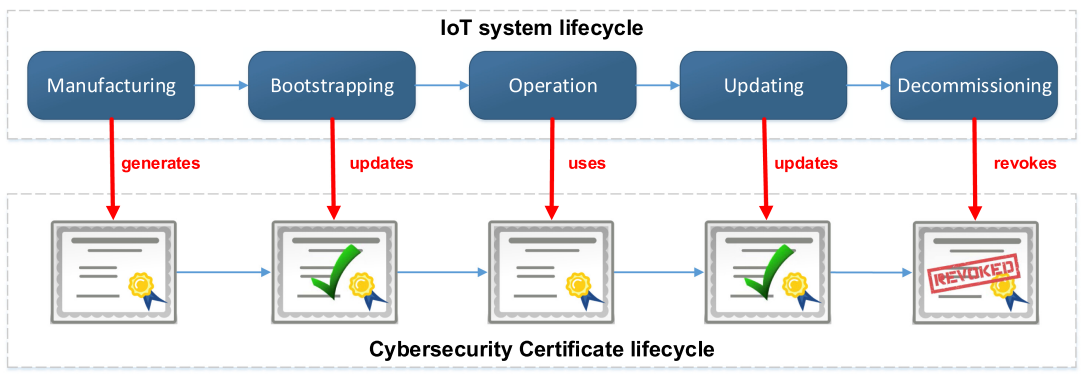
\includegraphics[scale=0.5]{images/lifeCycle.png}
    \caption{The cybersecurity certificate during the IoT device lifecycle.}
    \label{fig:lifecycle}
\end{figure}
As mentioned above, certificates are subject to invalidation, whether caused by a context change, a property change, or simply by the certificate's expiration; all certificates have a finite lifespan managed by the Certificate Authority (CA), which is usually also in charge of replacing it with a new one. However, the CA represents a bottleneck, and automation frameworks are needed when dealing with highly dynamic environments like Cloud and Edge. Therefore, the life cycle of a certificate is de facto a deterministic finite-state automaton whose state transitions are determined by specified conditions.

As mentioned above, certificates are subject to invalidation, whether caused by a context change, a property change, or simply by the certificate's expiration; all certificates have a finite lifespan managed by the Certificate Authority (CA), which is usually also in charge of replacing it with a new one. However, the CA represents a bottleneck, and automation frameworks are needed when dealing with highly dynamic environments like Cloud and Edge. Therefore, the life cycle of a certificate is de facto a deterministic finite-state automaton whose state transitions are determined by specified conditions. As shown in figure \ref{fig:lifecycle}, the lifecycle of a certificate is tightly coupled with the lifecycle of the IoT system, which is usually divided into five phases: i) Manufacturing, ii) Bootstrapping, iii) Operation, iv) Updating and v) Decommissioning. 

The manufacturing phase includes the production, programming and configuration of the system/device. This phase also includes the security certification process, which, if passed, assigns a brand new certificate to the system. The bootstrapping phase includes the installation and configuration of the device for the specific domain in which it will operate. Moreover, context-specific information should be embedded in the cybersecurity label (this step is too often ignored). It is also important to note that the context plays a fundamental role in every IoT system; a given device could require different security levels based on the type of information it needs to handle, and this variation can happen multiple times in the lifespan of the device. During the operation phase, the device/system provides its intended functionalities and should always be kept under a monitoring process. The monitoring is crucial to find new vulnerabilities and issues in the system. When a new vulnerability is found, and the manufacturer issues an update, rarely is a re-certification not issued due to the complexity of the analysis of the changes. Moreover, the security level and label are updated during a re-certification process. The decommissioning phase represents the end of the lifecycle of the system and includes the certificate revocation. This phase is also crucial because the devices composing the system could have stored sensitive information, and this phase's sole purpose is to make such information inaccessible \cite{surveyIOT}.

Typically, a certification process for Cloud services consists of a collaborative effort between four entities: i) a service provider who develops the service that needs to be certified, ii) a cloud provider supporting the service's certification, iii) a CA responsible for the definition of the requirements and the methodology and iv) an accredited lab to carry out the system evaluation. The problem of such an approach resides in the fact that continuous context changes can rapidly invalidate the assigned certificates, and without proper context testing techniques, it is necessary to re-certificate the whole service every time. The framework that M. Anisetti et al. proposed addressed this issue by constantly verifying the possessed certifications against the context changes to prevent unnecessary revocations and re-certifications.


\subsubsection{Labels}
Labelling schemes exist to straightforwardly inform the user about the security certification that has been executed on a device; such schemes should contain the following main groups of information:

\begin{itemize}
    \item Domain that was considered while performing the certification activity; the certification should be revoked the moment the device leaves it

    \item Level of assurance; states the security tests performed to certify the device. Usually, the level of assurance is associated with the protection profile of the specific domain

    \item  Information about the achievement of the certification, such as the responsible entity, the process and the validity period

\end{itemize}

Even though the importance of labels is mostly tied to commercial purposes \cite{baldini2016security}, perhaps, they could also be read by the Certification Authorities to have a quicker overview of the system's mechanisms and capabilities. In state-of-the-art schemes, labels are ignored or poorly used, but they might play a fundamental role in future schemes.


\subsection{Assurance for Highly Distributed Paradigms}
As described in section \ref{Edge}, Edge computing adds multiple challenges to the table in terms of functionalities, especially when combined with IoT layers, which bring on even more security and assurance topics. Mahmud et al. \cite{mahmud2018fog} highlighted three security aspects that will inherently haunt new highly distributed computing paradigms:
\begin{itemize}

\item Technological discoveries advance at different paces for software and hardware; new software architectures (like edge computing) are designed upon traditional components, especially for networking, raising the number of vulnerabilities to attacks.

\item Highly distributed systems make it difficult to ensure secure authentication and privacy in every node at all times; monitoring frameworks could be insufficient in many cases.

\item Security mechanisms for data-centric integrity can greatly affect the quality of service of these systems.

\end{itemize}


